\section{Ingestion module for the TLM\_REQ\_B\ files}

This section describes the ingestion module for inserting the telemetry files containing the memory information of the satellite.
The associated ingestion processor is 

\begin{itemize}
    \item \textbf{s2boa.ingestions.ingestion\_tlm\_req\_b.ingestion\_tlm\_req\_b}
\end{itemize}

This module uses the folowing \acrshort{dim} signatures:
\begin{itemize}
    \item \textbf{MEMORY\_EVOLUTION\_XXX}: data containing the evolution of the memory in the different storages (NOMINAL, NRT) for the two channels as well as the last replayed scene to ground for the two channels.
\end{itemize}

Where XXX is the corresponding satellite id.

The figure \ref{fig:structure_ingestion_tlm_req_b} shows a simplified diagram of the structure of events inserted (associated structure of values not included for simplicity).

\begin{figure}[H]
  \begin{center}
	\centering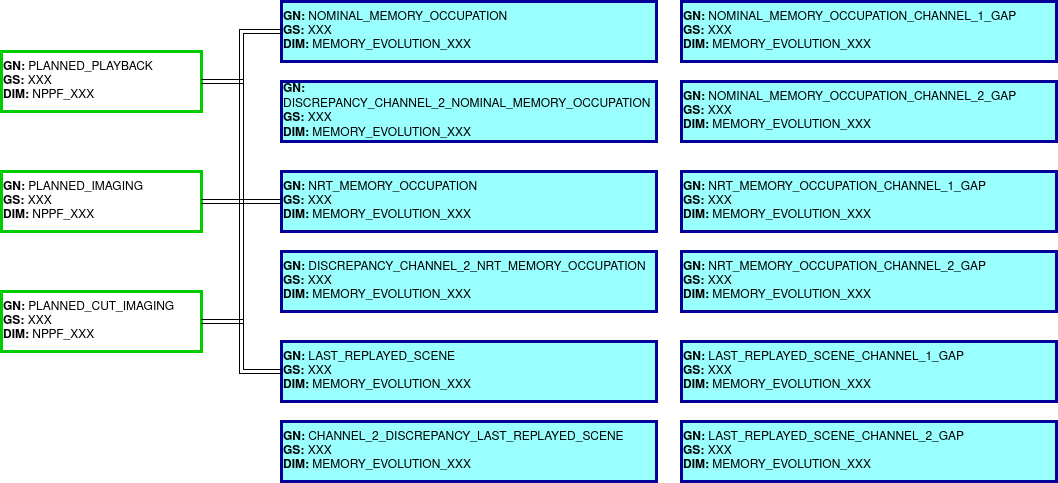
\includegraphics[width=170mm]{../fig/structure_ingestion_tlm_req_b.png}
	\caption{Structure of events inserted by the ingestion module for the TLM\_REQ\_B file}
	\label{fig:structure_ingestion_tlm_req_b}
  \end{center}
\end{figure}

The table \ref{tb:description_events_ingestion_tlm_req_b} shows the description of the events inserted by the ingestion module.
\begin{landscape}
    \begin{longtable}{|M{0.15\linewidth}|M{0.05\linewidth}|M{0.10\linewidth}|M{0.10\linewidth}|M{0.2\linewidth}|M{0.125\linewidth}|M{0.125\linewidth}|}
    \hline \textbf{Gauge name} & \textbf{Gauge system} & \textbf{DIM signature} & \textbf{Insertion mode} & \textbf{Description} & \textbf{Start} & \textbf{Stop} \\ \hline
    \textbf{NOMINAL\_MEMORY\_OCCUPATION} & XXX & \- MEMORY\_EVOLUTION\_XXX & INSERT\_and\_ERASE (insert\_and\_erase) & Event for representing the \textbf{NOMINAL memory evolution} taking as reference the values for channel 1& UTC time associated to a new engineering\_value & UTC time associated to the last instance of the same enineering\_value \\ \hline
    \textbf{DISCREPANCY\_CHANNEL\_2\_NOMINAL\_MEMORY\_OCCUPATION} & XXX & \- MEMORY\_EVOLUTION\_XXX & INSERT\_and\_ERASE (insert\_and\_erase) & Event for representing the \textbf{discrepancy between the NOMINAL memory occupation of Channel 1 and the NOMINAL memory occupation of Channel 2} & UTC time associated to the discrepancy & UTC time associated to the discrepancy \\ \hline
    \textbf{NRT\_MEMORY\_OCCUPATION} & XXX & \- MEMORY\_EVOLUTION\_XXX & INSERT\_and\_ERASE (insert\_and\_erase) & Event for representing the \textbf{NRT memory evolution} taking as reference the values for channel 1 & UTC time associated to a new engineering\_value & UTC time associated to the last instance of the same enineering\_value  \\ \hline
    \textbf{DISCREPANCY\_CHANNEL\_2\_NRT\_MEMORY\_OCCUPATION} & XXX & \- MEMORY\_EVOLUTION\_XXX & INSERT\_and\_ERASE (insert\_and\_erase) & Event for representing the \textbf{discrepancy between the NRT memory occupation of Channel 1 and NRT memory occupation of Channel 2} & UTC time associated to the discrepancy & UTC time associated to the discrepancy \\ \hline
    \textbf{LAST\_REPLAYED\_SCENE} & XXX & \- MEMORY\_EVOLUTION\_XXX & INSERT\_and\_ERASE (insert\_and\_erase) & Event for representing the \textbf{last replayed scene} taking as reference the values for channel 1 & UTC time associated to a new engineering\_value & UTC time associated to the last instance of the same enineering\_value  \\ \hline
    \textbf{DISCREPANCY\_CHANNEL\_2\_LAST\_REPLAYED\_SCENE} & XXX & \- MEMORY\_EVOLUTION\_XXX & INSERT\_and\_ERASE (insert\_and\_erase) & Event for representing the \textbf{discrepancy between the last replayed scene of Channel 1 and the last replayed scene of Channel 2} & UTC time associated to the discrepancy & UTC time associated to the discrepancy  \\ \hline
    \textbf{NOMINAL\_MEMORY\_OCCUPATION\_CHANNEL\_1\_GAP} & XXX & \- MEMORY\_EVOLUTION\_XXX & INSERT\_and\_ERASE (insert\_and\_erase) & Event for representing the \textbf{gaps in the NOMINAL memory occupation of Channel 1} of more than 6 seconds & UTC time associated to the beginning of the gap & UTC time associated to the end of the gap  \\ \hline
    \textbf{NOMINAL\_MEMORY\_OCCUPATION\_CHANNEL\_2\_GAP} & XXX & \- MEMORY\_EVOLUTION\_XXX & INSERT\_and\_ERASE (insert\_and\_erase) & Event for representing the \textbf{gaps in the NOMINAL memory occupation of Channel 2} of more than 6 seconds& UTC time associated to the beginning of the gap & UTC time associated to the end of the gap  \\ \hline
    \textbf{NRT\_MEMORY\_OCCUPATION\_CHANNEL\_1\_GAP} & XXX & \- MEMORY\_EVOLUTION\_XXX & INSERT\_and\_ERASE (insert\_and\_erase) & Event for representing the \textbf{gaps in the NRT memory occupation of Channel 1} of more than 6 seconds& UTC time associated to the beginning of the gap & UTC time associated to the end of the gap  \\ \hline
    \textbf{NRT\_MEMORY\_OCCUPATION\_CHANNEL\_2\_GAP} & XXX & \- MEMORY\_EVOLUTION\_XXX & INSERT\_and\_ERASE (insert\_and\_erase) & Event for representing the \textbf{gaps in the NRT memory occupation of Channel 2} of more than 6 seconds& UTC time associated to the beginning of the gap & UTC time associated to the end of the gap  \\ \hline
    \textbf{LAST\_REPLAYED\_SCENE\_CHANNEL\_1\_GAP} & XXX & \- MEMORY\_EVOLUTION\_XXX & INSERT\_and\_ERASE (insert\_and\_erase) & Event for representing the \textbf{gaps in the last replayed scene data of Channel 1} of more than 6 seconds& UTC time associated to the beginning of the gap & UTC time associated to the end of the gap  \\ \hline
    \textbf{LAST\_REPLAYED\_SCENE\_CHANNEL\_2\_GAP} & XXX & \- MEMORY\_EVOLUTION\_XXX & INSERT\_and\_ERASE (insert\_and\_erase) & Event for representing the \textbf{gaps in the last replayed scene data of Channel 2} of more than 6 seconds& UTC time associated to the beginning of the gap & UTC time associated to the end of the gap  \\ \hline
    \caption{Table describing the events associated to the ingestion}
    \label{tb:description_events_ingestion_tlm_req_b}
    \end{longtable}
    \end{landscape}